\chapter{Full Visual Odometry}
% Title ideas: 
% Visual Odometry with Deep Learning
% Visual Odometry
% The Full Visual Odometry Pipeline

	\section{Introduction}
	% Describe the Task
	% Prior Work -> Flownet, DeepVO, VINet
	%
	The bulk of this chapter and the following experiments are based on the work of \cite{wang2017deepvo}.
	At the time of writing this thesis, \citeauthor{wang2017deepvo} have not released the source code of their implementation.
	Therefore, the aim of this chapter is to study and re-implement the ideas presented in their paper and to further expand on it.
	
	\section{Datasets}
		\todo{intro text}
		\begin{figure}
			\centering
			\begin{subfigure}[b]{0.8\linewidth}
				\centering
				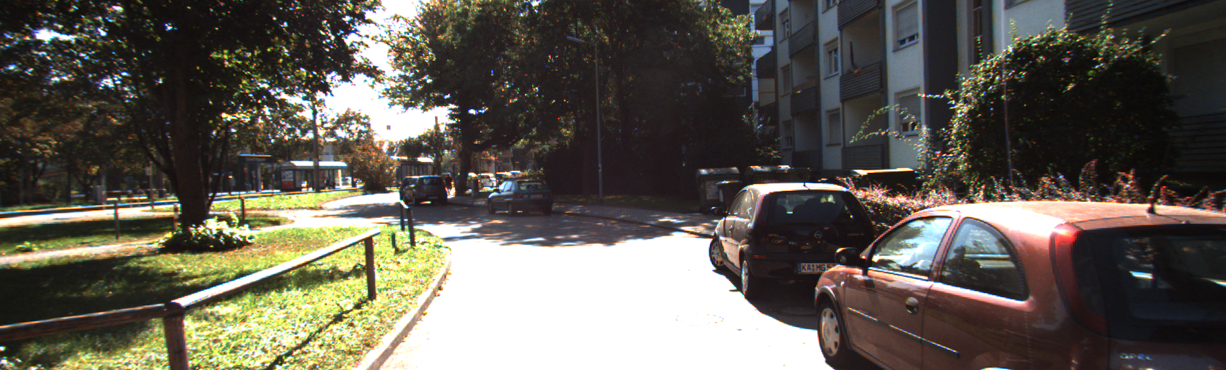
\includegraphics[width=\linewidth]{Data/kitti-example-image}
				\caption{
					KITTI
					\label{fig:kitti-example-image}
				}
			\end{subfigure}%
			\\
			\begin{subfigure}[b]{0.8\linewidth}
				\centering
				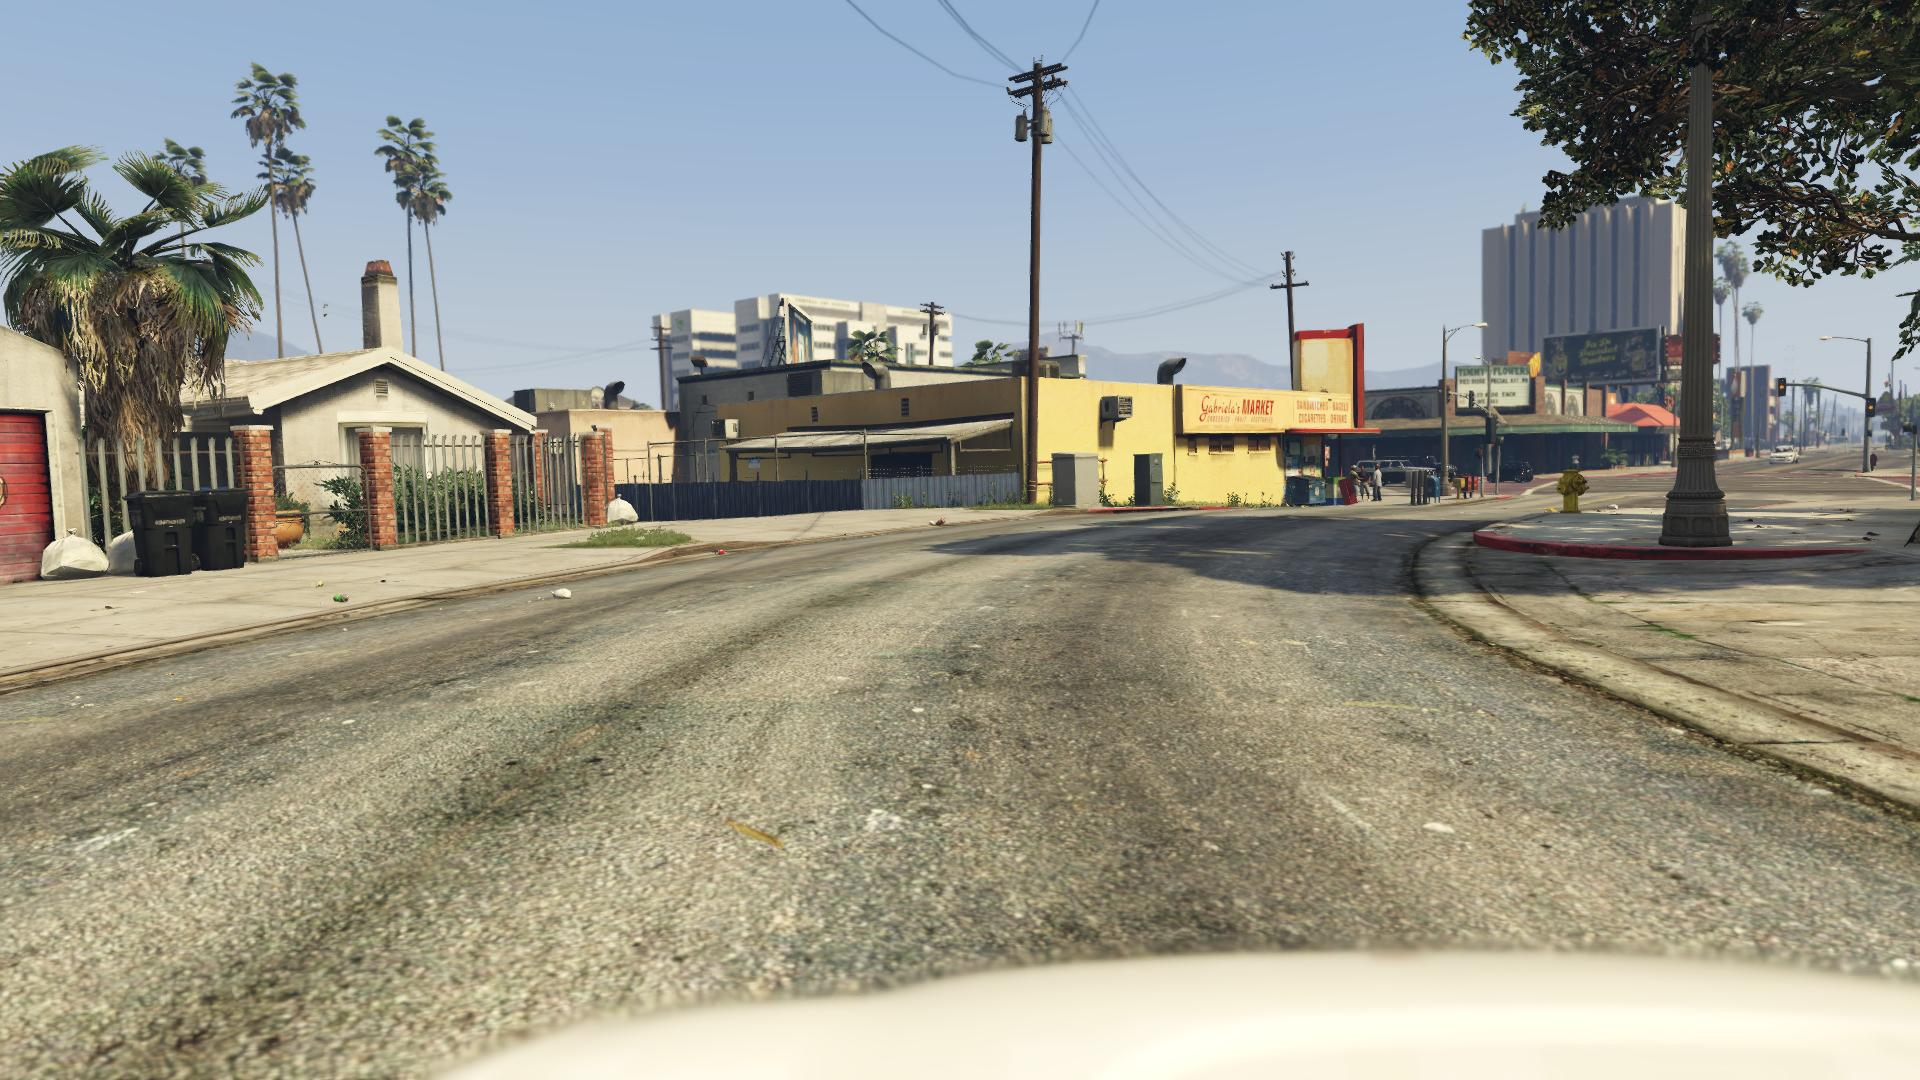
\includegraphics[width=\linewidth]{Data/viper-example-image}
				\caption{
					VIPER
					\label{fig:viper-example-image}
				}
			\end{subfigure}%
			\caption[Example images from different datasets]
					{Example images from different datasets.
					 \todo{choose different image with scene dynamics, and show more images per dataset}
					 \label{fig:example-images-from-datasets}}
		\end{figure}
		\subsection{KITTI}
			KITTI from Karlsruhe Institute of Technology \cite{geiger2013vision} is a dataset that contains many video frames captured from the roof of a driving car.
			Each video frame is labeled with ground truth data such as camera pose and 3D points from a velodyne laser scanner.
			The camera pose was obtained by combining the data from GPS and an IMU (inertial measurement unit) that was mounted to the car.
			The dataset has around 23k stereo pairs of images with size $1226 \times 370$ pixels captured at a frame rate of [FPS]\todo{find frame rate}.
			For the experiments in this thesis, only the images from the left camera are used.
			The dataset is divided into 22 sequences, each captured at a different location in the metropolitan area of Karlsruhe, Germany.
			For the public, the ground truth is only available for the first 11 sequences.
			The rest of the data is intended to be used for submissions to the KITTI Vision Benchmark Suite\footnote{\url{http://www.cvlibs.net/datasets/kitti/eval_odometry.php}} 
			online.
			In the experiments here, only the sequences 0 to 10 are used and divided into training- and test sets.
		
		\subsection{VIPER}
			The VIPER dataset \cite{richter2017playing} contains a mix of car driving and walking sequences, but all data was generated synthetically from the video game Grand Theft Auto 5 released in April 2015.
			With around 254k frames it is significantly larger that the KITTI dataset.
			There is a variety of ground truth data available, including camera pose, semantic class labels and 3D object bounding boxes.
			The camera poses have been directly extracted from the game engine and are therefore fully accurate, while other data such as the semantic labels were generated in a post-processing step.
			VIPER is subdivided into training, test, and validation sets with 134k, 70k, and 50k frames respectively.
			The splits contain diverse scenes at day and night across different scene types such as urban, suburban under various weather conditions.
			
		\subsection{GTA V}
		% Self made dataset
		% mention that code for viper is not available
		% link to github repository
		% explain how it was caputured
		% What type of data does it contain
		%	- walking, running, driving, standing, 
		%	- weather, light, dynamic scene
		%	- 
		
		\subsection{Preprocessing}\label{sec:preprocessing}
			Each dataset contains long sequences/videos of thousands of frames over several minutes of recording.
			Due to the high memory footprint, it is unfeasible to load a complete sequence and feed it to the network.
			Therefore the sequences are cut into subsequences of smaller sizes. 
			For most experiments here, the sequence size is 100 frames or less.
			Instead of creating a segmentation of the dataset, this method of extracting subsequences also allows to define an overlap between sequences.
			This is especially useful when the dataset is small, such as KITTI.
			
			Since resolution and aspect ratio of the images are different between the datasets, they are first proportionally resized to a height of 320 pixels and then the center region of $448 \times 320$ pixels is extracted.
			Fixing the input size across multiple datasets makes it possible to train the same network architecture for different data and make a more accurate comparison.
			Due to the cropping, the left and right boundaries of the image are removed.
			An alternative is to resize the images directly without regard to the aspect ratio.
			This leads to a loss in horizontal resolution which could impact the networks performance for horizontal motions, e.g., a rotation of the camera around the vertical axis.
			The alternative resizing method was not studied in this thesis, but the impact is expected to be minor.
			
			The ground truth poses also require preprocessing. 
			Each raw sequence has a corresponding text file that contains the $3 \times 4$ pose matrices for every frame.
			These poses are all relative to the coordinate system of the first frame in the sequence.
			In other words, the coordinate system of the first frame is the world coordinate system of all other frames in the sequence.
			Because the raw sequences are divided into subsequences, the ground truth poses need to be converted to poses that are relative to the first frame within each subsequence.
			\todo{Refer to math equations in introduction}
			
			
	\section{Encoding the Pose}
	% Text from intro
	
	
	\section{The Model}
	% Figure with the entire pipeline
	% - Figure showing optical flow ??
	% Feature extraction
	%	- Optical flow
	%	- features relevant for motion
	%	- Flow alone is not enough
	% 	- Other high-level representation
	% Pose estimation
	%	- LSTM transforms feature to pose
	%	- Uses history from poses seen before to make current estimate more precise
	%	- 
	% Loss function and optimization
	% mse loss on euler + translation
	% experiments show that euler works best
	% 	
		The model is the key to solving the task.
		By adjusting the weights during the training phase, it learns a high-level representation of relevant information in the input that is needed to produce the desired output.
		In the case of visual odometry, we aim to learn a representation for motion.
		Specifically, the network has to be able to distinguish between dynamic motion in the scene and camera motion.
		\todo{Refer to challenges/ambiguities discussed in introduction...}
		The following two sections describe the two main parts of the model.
		The architecture of the full model is shown in figure~\ref{fig:main-architecture}.
		\begin{figure}[t]
			\centering
			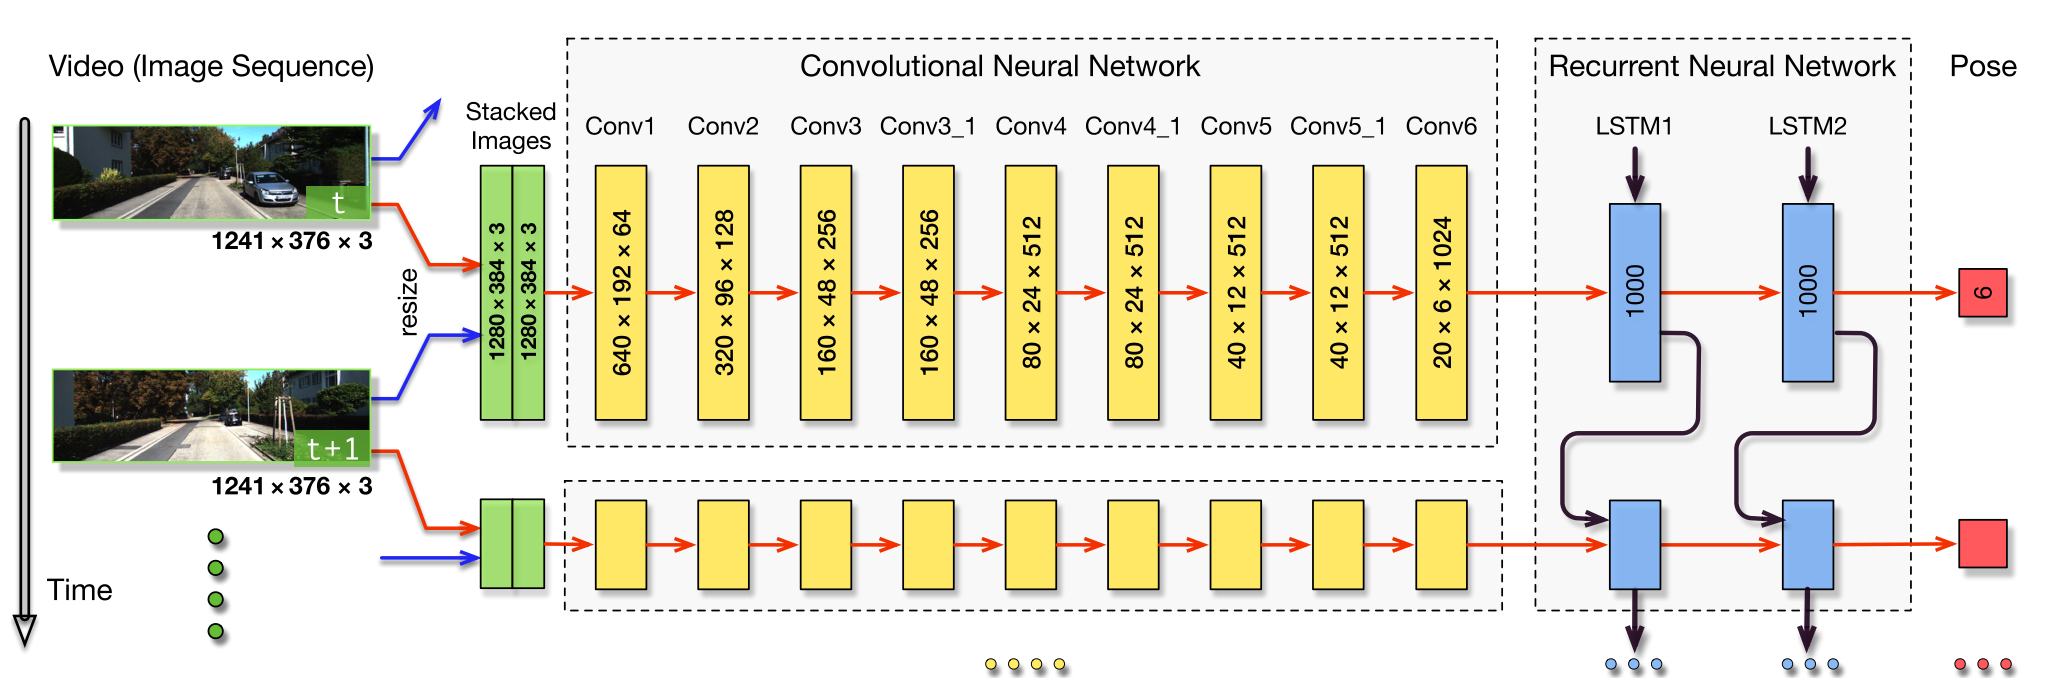
\includegraphics[width=\linewidth]{Model/DeepVO-arch}
			\caption[Main architecture for visual odometry]
					{Main architecture for visual odometry.
					 Green: Input of consecutive frames.
					 Yellow: Feature extraction.
					 Blue: Pose estimation with recurrent connections.
					 \todo{ref paper for figure, or redo figure}
					 \label{fig:main-architecture}}
		\end{figure}
		
		\subsection{Part 1: Feature Extraction}
			The purpose of the first part of the network is to extract information about motion from two consecutive frames at time $t$ and $t - 1$.
			One way to describe motion between two images is by \emph{optical flow}.
			It is defined as a vector-valued function $u(\vectr{x}) \in \R^2$ at each point $\vectr{x}$ in the image $I_{t}$ describing the translation of the point in the next frame such that
			\begin{equation}\label{eq:brightness_constancy_constraint}
				I_{t}(\vectr{x}) = I_{t + 1}(\vectr{x} + u(\vectr{x})).
			\end{equation}
			The property in equation~\ref{eq:brightness_constancy_constraint} is called the \emph{brightness constancy constraint}. 
			It means that a particular point can move in the image plane but it does not change its color.
			In general, this constraint does not hold for every point, e.g., because of occlusion introduced by motion.
			
			\cite{dosovitskiy2015flownet} describe a deep-learning approach for estimating optical flow.
			They propose and study two network architectures, \emph{FlowNetS} and \emph{FlowNetC}.
			The later is computing the inner product between patches of two input frames (correlation) followed by multiple layers of convolutions.
			FlowNetS on the other hand is the simple version that does not have the correlation layer. 
			Instead, it is only made of convolution layers and ReLUs.
			The first half of FlowNetS are strided convolutions that gradually increase the number of feature maps. 
			The second half, called refinement, consists of transposed convolution layers that, in reverse, increase the spatial dimension to form the high resolution optical flow maps.
			In addition, both FlowNet versions make use of skip-connections that allow the features from earlier layers to be added as input to layers in the second half by concatenating the tensors along the feature channel dimension. 
			
			In this thesis, the focus is on FlowNetS because it is the only publicly available implementation for PyTorch.\footnote{\citet*{flownetpytorch} has the source code available on GitHub.}
			FlowNetS is also the choice in the work of \citeauthor{wang2017deepvo}, which is the basis of the architecture described here.
			The FlowNetS implementation comes with pre-trained model weights.
			It is trained on a synthetic dataset of moving chairs rendered into images that serve as a static background.
			Although this data does not include camera motion, according to \citeauthor{wang2017deepvo} the model weights serve as a good initialization that leads to faster convergence. 
			
			Estimating camera motion solely based on optical flow is not very robust since scene motion is mixed into the optical flow which can significantly vary in magnitude.
			In order to have a more abstract representation, only the layers in the first half up to ``conv6.1'' are used for feature extraction.
			All layers in the second half of FlowNetS are dropped.
			The exact configuration of the remaining layers is shown in table~\ref{tbl:first_part_of_flownets}.
			\begin{table}[tb]
				\small
				\begin{center}
					\begin{tabular}{|l|c|c|c|c|}
						\hline
						Layer 		& Kernel size 		& Stride 		& Padding 		& Channels 		\\ \hline
						conv1 		& $7 \times 7$		& 2 			& 3 			& 64 			\\ \hline
						conv2 		& $5 \times 5$		& 2 			& 2 			& 128 			\\ \hline
						conv3 		& $5 \times 5$		& 2 			& 2 			& 256			\\ \hline
						conv3.1 	& $3 \times 3$		& 1 			& 1 			& 256 			\\ \hline
						conv4 		& $3 \times 3$		& 2 			& 1 			& 512 			\\ \hline
						conv4.1 	& $3 \times 3$		& 1 			& 1 			& 512 			\\ \hline
						conv5 		& $3 \times 3$		& 2 			& 1 			& 512 			\\ \hline
						conv5.1 	& $3 \times 3$		& 1 			& 1 			& 512 			\\ \hline
						conv6 		& $3 \times 3$		& 2 			& 1 			& 1024 			\\ \hline
						conv6.1 	& $3 \times 3$		& 1 			& 1 			& 1024 			\\ \hline
					\end{tabular}
				\end{center}
				\caption[Architecture of the feature extraction based on FlownetS]
						{Architecture of the feature extraction based on FlownetS. 
						 Each layer is a convolution followed by a rectified linear unit (ReLU).
						 \label{tbl:first_part_of_flownets}}
			\end{table}
			Note that the convolutions are applied with a stride and therefore the spatial size is reduced from one layer to the next.
			At the same time, the number of feature maps (channels) increases up to 1024 in the last layer.
			Say the input images have a width and height of $448 \times 320$ pixels, for example. 
			Then the output tensor contains 1024 feature maps of size $7 \times 5$.
			These activations are a coarse and abstract description of the motion seen in the input and do not directly imply the per-pixel optical flow.
			To emphasize again, we do not directly make use of optical flow since we are interested in separating camera motion from scene motion.
			This has to be done on a higher level of abstraction.
			The remaining task is now to take these coarse features and map them to the camera pose. 
			
		\subsection{Part 2: Pose Estimation}
		% How does LSTM use flow features 
		% Table with fc layer and dropout
			The key component of the second part is the LSTM that maps the motion features to a hidden state.
			Due to the recurrent connections, the hidden state does not only encode the pose at the current time step, but also a history of poses from previous time steps.
			To be clear, it is not obvious that the LSTM will actually learn a representation for the past and use that information to estimate the pose because nothing is explicitly forcing the network to do so.
			The question whether or not the recurrent connections make a significant contribution will be addressed in section~\ref{sec:odometry-experiments-and-results}.
			
			As opposed to convolution layers, the LSTM is defined in terms of matrix operations and hence the size of the input to the LSTM is not variable.
			This also implies that there is a limit on the size of the input images.
			As described in section~\ref{sec:preprocessing}, the images are rescaled to $448 \times 320$ pixels, which leads to a tensor of size $1024 \times 7 \times 5$ after feature extraction.
			This tensor is then reshaped to a vector with $1024 \cdot 7 \cdot 5 = 35840$ elements and fed to the LSTM as input.
			Although the LSTM itself applies multiple operations involving input, hidden state and gate outputs, it can be summarized as one single layer.
			Moreover, as shown in figure~\ref{fig:main-architecture} we adopt the architecture of~\citeauthor{wang2017deepvo} and stack two LSTM layers.
			Each of these recurrent layers has an associated hidden state of size $d = 1000$.
			
			The recurrent layers are followed by dropout and a fully connected layer that reduces the output size of the LSTM to a 6D vector for the pose.
			Table~\ref{tbl:lstm_and_fc_after_flownet} summarizes the input- and output dimensions of all layers in the second component of the network.
			\begin{table}[tb]
				\small
				\begin{center}
					\begin{tabular}{|l|c|c|}
						\hline
						Layer 		& Input size 					& Output size			\\ \hline
						lstm1 		& $35840$						& $1000$  				\\ \hline
						lstm2 		& $1000$						& $1000$ 				\\ \hline
						drop		& $1000$						& $1000$				\\ \hline
						fc 			& $1000$						& $6$					\\ \hline
					\end{tabular}
				\end{center}
				\caption[Architecture of the recurrent part of the pose network]
						{Architecture of the recurrent part of the pose network.
						 It consists of a two-layer LSTM with hidden size 1000, a dropout- and fully-connected layer.}
				\label{tbl:lstm_and_fc_after_flownet}
			\end{table}
		
		\subsection{Loss Function}
			At each time step $t = 1, \dots, T$ the LSTM outputs a pose estimate 
			$\vectr{\hat{y}}_t = \left[ \, \vectr{\hat{p}}_t,  \vectr{\hat{\varphi}}_t \right]$.
			The quality of this estimate is compared against the ground truth pose 
			$\vectr{y}_t = \left[ \, \vectr{p}_t,  \vectr{\varphi}_t \right]$
			with the loss function
			\begin{equation}\label{eq:euler_pose_loss_function_t}
				\mathcal{L}_t(\vectr{y}_t, \vectr{\hat{y}}_t) = 
				%\sum_{t=1}^{T} 
					\lVert \vectr{p}_t - \vectr{\hat{p}}_t \rVert_2^2 + 
					\beta \lVert \vectr{\varphi}_t - \vectr{\hat{\varphi}}_t \rVert_2^2.
			\end{equation}
			This loss function balances the squared error of position and Euler angles with a factor $\beta$.
			The scale of positional change is usually higher than the angular changes for rotation, but in general, the scale depends on the ground truth provided in the dataset, e.g., the unit of measurements used or the speed of the camera motion.
			The balance factor $\beta$ is part of the hyper parameters and has to be fixed before training. 
			\todo{Mention choice of beta in experiments section}
			
			
			
	\section{Experiments and Results}\label{sec:odometry-experiments-and-results}
	% Ablation studies
	% Problem with "global" pose -> incremental pose
	% Training
	%	- Different learning rate for pretrained flownet
	%	- Dropout Regularization
	
		\begin{table}[tb]
			\small
			\begin{center}
				\begin{tabular}{|c|c|c||c|c|c|}
					\hline
					Length 	& Overlap 	& Dropout	& Total 	& Rotation	& Translation	\\ \hline
					25		& 0			& 0			& 19.0293	& 0.4981	& 18.5312		\\ \hline
					25		& 20		& 0			& 16.5471	& 0.3913	& 16.1558		\\ \hline
					100		& 20		& 0			& 529.9459	& 39.8967	& 490.0493		\\ \hline
					100 	& 5			& 0.5		& 376.7666	& 43.1578	& 333.6088		\\ \hline
					100		& 80		& 0			& 313.1278	& 47.8437	& 265.2841		\\ \hline
				\end{tabular}
			\end{center}
			\caption[Experiments on KITTI: Overlap and dropout]
					{Experiments on KITTI: Overlap and dropout. 
					 Shown is the test error on sequence 10 for different overlap and dropout during training.
					 Each model was trained with default parameters for 100 epochs.
					 \todo{also include growing sequence?}
					 \label{tbl:kitti-overlap-and-dropout}}
		\end{table}
		
		\begin{table}[tb]
			\small
			\begin{center}
				\begin{tabular}{|c|c||c|c|c|}
					\hline
					Training length & Test length 	& Total 	& Rotation	& Translation	\\ \hline
					25				& 25			& 16.5471	& 0.3913	& 16.1558		\\ \hline
					25				& 100			& 1060.7528	& 37.6196	& 1023.1332		\\ \hline
					100				& 100			& 529.9459	& 39.8967	& 490.0493		\\ \hline
				\end{tabular}
			\end{center}
			\caption[Experiments on KITTI: Testing on longer sequences]
					{Experiments on KITTI: Testing on longer sequences. 
					 When testing on longer sequences, the error becomes extremely high compared to the model trained on 100 frames.
					 \label{tbl:kitti-testing-on-longer-sequences}}
		\end{table}
	
		\begin{figure}
			\centering
			\begin{subfigure}[b]{0.5\linewidth}
				\centering
				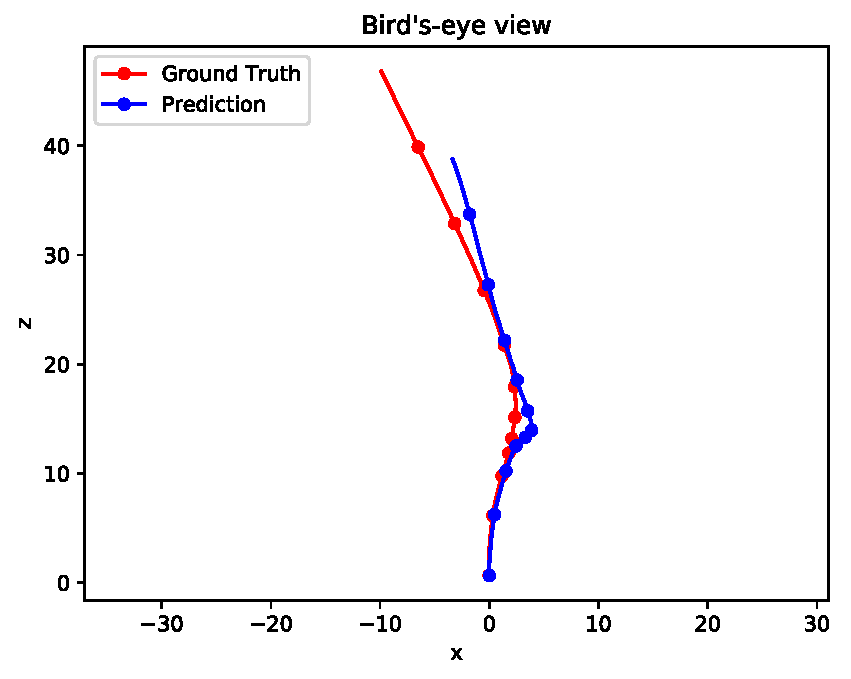
\includegraphics[width=\linewidth]{Images/Experiments/trained-on-25-frames}
				\caption{
					\label{fig:0}
				}
			\end{subfigure}%
			\begin{subfigure}[b]{0.5\linewidth}
				\centering
				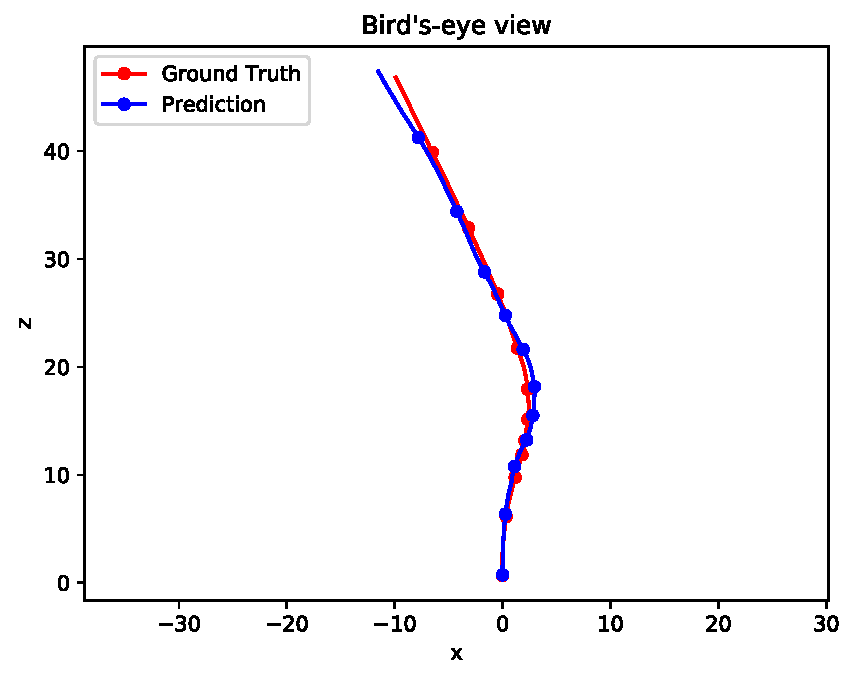
\includegraphics[width=\linewidth]{Images/Experiments/trained-on-100-frames}
				\caption{
					\label{fig:1}
				}
			\end{subfigure}%
			\caption[Training and testing on different sequence length]
					{Training and testing on different sequence length. 
					 Two models tested on a KITTI subsequence of 100 frames and trained on sequences of (a) 25 frames and (b) 100 frames. 
					 The markers in the plot are shown every ten frames.
					 \label{fig:kitti-testing-on-longer-sequences}}
		\end{figure}
	
		\begin{figure}
			\centering
			\begin{subfigure}[b]{\linewidth}
				\centering
				\includegraphics[width=0.45\linewidth]{example-image-a}
				\includegraphics[width=0.45\linewidth]{example-image-a}
				\caption{
					Long, curve
					\label{fig:0}
				}
			\end{subfigure}%
			\\
			\begin{subfigure}[b]{\linewidth}
				\centering
				\includegraphics[width=0.45\linewidth]{example-image-b}
				\includegraphics[width=0.45\linewidth]{example-image-b}
				\caption{
					Short
					\label{fig:0}
				}
			\end{subfigure}%
			\\
			\begin{subfigure}[b]{\linewidth}
				\centering
				\includegraphics[width=0.45\linewidth]{example-image-c}
				\includegraphics[width=0.45\linewidth]{example-image-c}
				\caption{
					\label{fig:0}
				}
			\end{subfigure}%
			\caption[Qualitative results for motion estimation on KITTI]
					{Qualitative results for motion estimation on KITTI.
					 Left column: Visualization of the estimated and true path.
					 Right column: Plot of each coordinate axis.
					 Markers are shown for every \todo{xx} frames.
					\label{fig:0}}
		\end{figure}
	
	
		\begin{figure}
			\centering
			\begin{subfigure}[b]{\linewidth}
				\centering
				\includegraphics[width=0.45\linewidth]{example-image-a}
				\includegraphics[width=0.45\linewidth]{example-image-a}
				\caption{
					Long, curve
					\label{fig:0}
				}
			\end{subfigure}%
			\\
			\begin{subfigure}[b]{\linewidth}
				\centering
				\includegraphics[width=0.45\linewidth]{example-image-b}
				\includegraphics[width=0.45\linewidth]{example-image-b}
				\caption{
					Short
					\label{fig:0}
				}
			\end{subfigure}%
			\\
			\begin{subfigure}[b]{\linewidth}
				\centering
				\includegraphics[width=0.45\linewidth]{example-image-c}
				\includegraphics[width=0.45\linewidth]{example-image-c}
				\caption{
					\label{fig:0}
				}
			\end{subfigure}%
			\caption[Qualitative results for motion estimation on VIPER]
					{Qualitative results for motion estimation on VIPER.
					 \label{fig:0}}
		\end{figure}
		
	\section{Discussion}
	\section{Conclusion}
